\documentclass[a4paper,12pt]{article}
\usepackage{amsmath,amsfonts,amssymb,graphicx,hyperref,dcolumn}
\setcounter{MaxMatrixCols}{30}
\newtheorem{theorem}{Theorem}
\newtheorem{remark}[theorem]{Remark}
\newenvironment{proof}[1][Proof]{\noindent\textbf{#1.} }{\ \rule{0.5em}{0.5em}}
\def\NOMDOSSIER{DB$\cdot$nomics with\\MATLAB}
\def\NUMERODOSSIER{0}

%\input{../lectures_info.tex}
% basic  stuff
\usepackage[T1]{fontenc}
\usepackage{lmodern}
\usepackage{graphicx}
\usepackage{color}
\usepackage{xcolor}
\usepackage{hyperref}
\usepackage{eurosym}
\usepackage{natbib}
\usepackage{minted}
\usepackage[most]{tcolorbox}
\usetikzlibrary{calc}
\definecolor{deepblue}{RGB}{0,129,188}
\definecolor{deepblue2}{RGB}{0,26,153}
\definecolor{deepgreen}{RGB}{73,155,202}
\definecolor{mygray}{gray}{0.9}
\definecolor{myblue}{RGB}{0,163,243}

% the page size
\usepackage{geometry}
\geometry{a4paper, top=1.5cm, left=1cm, right=1.0cm, bottom=1.0cm, includehead, includefoot}
\graphicspath{{../},{../../},{/chap1},{/chap2},{/chap3},{/chap4},{/chap5},{/chap6},{../2018_macroeconometrics/}}
\pdfoptionpdfinclusionerrorlevel=0


% TOC programming
\usepackage{tocloft}
\setlength{\cftbeforesecskip}{2pt}
\setcounter{tocdepth}{1} % hide subsection in TOC

%%% BULLET LIST ITEMS
\usepackage{bm}
\newcommand{\localtextbulletone}{\textcolor{deepblue2}{\bm{$\circ$}}}
\renewcommand{\labelitemi}{\localtextbulletone}

% section programming 
\usepackage[calcwidth]{titlesec}
\titleformat{\section}% sectioning command formatted
            {\bfseries\LARGE\color{deepblue2}}% font commands applied to whole
            {\thesection .}% label
            {0.5em}% separation between label and title
            {}% commands before section title
            [{\titlerule[1pt]}]% commands after

\titleformat{\part}% sectioning command formatted
            {\bfseries\large}% font commands applied to whole
            {PARTIE \thepart ~:}% label
            {0.5em}% separation between label and title
            {}% commands before section title
            [{\titlerule[1pt]}]% commands after
			
%\renewcommand{\questionshook}{%
%   \setlength{\labelsep}{6pt}%  --> espace entre la puce et le début du texte
%    \setlength{\leftmargin}{0pt}%  --> espace entre le texte et la marge gauche (sauf pour la premiere ligne)
%    \setlength{\labelwidth}{30pt}% --> taille de la boite contenant la puce. Aligné à droite. Si taille < taille de la puce, la taille de la boite est egale à la taille de la puce
%   \setlength{\listparindent}{\parindent}% --> indentation des paragraphe dans la liste
%    \setlength{\itemindent}{30pt}% --> espace entre la marge et la puce
    %\setlength{\itemsep}{0pt}% --> espace entre les items (auquel s'ajoute \parsep}
%}
%\renewcommand\thequestion{\arabic{question}}
%\renewcommand{\questionlabel}{Question No.~\thequestion.}

%Pdf HYPPERREF STUFF
\hypersetup{
colorlinks=false,
	breaklinks=true,
	plainpages=false,
	%pdftitle={\letitre},
	pdfauthor={University of Paris-Dauphine},
	pdfsubject={},
	pdfcreator={TeX et TXC},
	%pdfstartpage={1},
	%pdfpagemode={FullScreen}
	pdfkeywords={DSGE, Business Cycles},
	pdfborder={0 0 0},
	bookmarksnumbered=true,
	pdfproducer={University Paris-Dauphine},     
	pdfnewwindow=true,          
	colorlinks=true,           
	linkcolor=deepblue,              
	citecolor=deepblue,            
	filecolor=black,          
	urlcolor=deepblue2 
}

% DEALING WITH BOXES
\usepackage{tcolorbox}
\newtcolorbox{mybox}[1]{colback=black!5,colframe=black!40,fonttitle=\bfseries,title=#1,fontlower=\sfdefault}
\newtcolorbox{myconsole}[1]{colback=deepblue!5,colframe=deepblue!40,fonttitle=\bfseries,title=#1,fontlower=\sfdefault}
\newtcolorbox{myresult}[1]{colback=black!5,colframe=deepgreen,fonttitle=\bfseries,title=#1,fontlower=\sfdefault}


%%% EXERCISE BOX
\newtcolorbox[auto counter]{assignment}{
  breakable,
  fonttitle=\bfseries,
  title={Assignment \thetcbcounter}
}
\newtcolorbox[auto counter]{myexercise}[1]{
  skin=enhanced,
  breakable,
  colback=white,
  colframe=gray!30,
  coltitle=black,
  fonttitle=\bfseries,
  leftrule=0.5cm,
  arc=0pt,
  outer arc=0pt,
  title={Exercise \thetcbcounter : #1}
}
\newtcolorbox{definitioniii}[1]{
  skin=enhanced,
  breakable,
  fonttitle=\bfseries,
  colback=white,
  arc=0pt,
  outer arc=0pt,
  title={#1},
  shadow={1mm}{-1mm}{0mm}{fill=gray,opacity=0.5,sharp corners}
}

% DEALING WITH THE EXAM CLASS
%\printanswers % If you want to print answers
% \noprintanswers % If you don't want to print answers
%\addpoints % if you want to count the points
% \noaddpoints % if you don't want to count the points
% Specifies the way question are displayed:
%\qformat{\textbf{Question \thequestion}\hfill}%\quad(\thepoints)\hfill}
%\definecolor{SolutionColor}{rgb}{0.8,0.9,1} % light blue
%\shadedsolutions % defines the style of the solution environment
% \framedsolutions % defines the style of the solution environment
% Defines the title of the solution environment:
%\renewcommand{\solutiontitle}{\noindent\textbf{Solution:}\par\noindent}
%\renewcommand{\questionlabel}{\textbf{~\thequestion)} }

% Table of content
\usepackage{titlesec}
\usepackage{titletoc}
\usepackage[titletoc]{appendix}
\contentsmargin{0pt}
\renewcommand\contentspage{\color{deepblue2}p. \thecontentspage}
\dottedcontents{section}[2.3em]{}{2.3em}{5pt}
\dottedcontents{subsection}[5.5em]{}{3.2em}{5pt}
\renewcommand*\contentsname{\bfseries\color{deepblue2}Content of the Handout}

% FRONT PAGE STUFF
\usepackage{setspace}
\def\FRONTPAGE{%
\begin{picture}(0,0)\unitlength=1cm
%\put (1,0) {\includegraphics[width=7.5em]{PSL.png}}
\put (7.5,-1.4) {
\includegraphics[width=.6\textwidth]{logo-upd.png}}
\end{picture}
\begin{center}
	\color{black!70}
	\ifnum\NUMERODOSSIER<1
		\rule{19cm}{.2pt}\\ \hfill Gauthier Vermandel \textcolor{deepblue2}{\bm{$\circ$}} \textit{gauthier.vermandel@dauphine.psl.eu} \\
		\vspace{2cm}
	\else
		\rule{19cm}{.2pt}\\ \hfill \the\year \\
		\textbf{\large \LECTURENAME }\\
		\vspace{0.5cm}
		\UNIV \\ \DIPLOMA \\
		\vspace{0.5cm}
		Gauthier Vermandel\footnote{Department of Economics, Paris-Dauphine University. Updated slides and codes available on my website: \WEBPAGE.} \hfill \textit{gauthier.vermandel@dauphine.fr} \\
		\rule[0.25cm]{19cm}{.2pt}\\
		\vspace{1cm}
	\fi
	\color{black}
  \ifnum\NUMERODOSSIER<1
	\ifnum\NUMERODOSSIER=0
		\begin{spacing}{1.25}
			\hspace{-.2cm}\textcolor{deepblue2}{\Large\textsc{A Note on}\\\textbf{\LARGE \NOMDOSSIER }}
		\end{spacing}
	 \else
		\begin{spacing}{1.25}
			\hspace{-.2cm}\textcolor{deepblue2}{\textbf{\LARGE \NOMDOSSIER }}
		\end{spacing}	 
	\fi
  \else
	\begin{center}
		\begin{minipage}{0.5\textwidth}
				\centering \textcolor{deepblue2}{ \hspace{-.23cm}\Large \textsc{ Chapter \NUMERODOSSIER }}\\ 
				\vspace{1ex}
		\end{minipage}
		 \\ \vspace{2ex}
		\begin{minipage}{0.65\textwidth}
				\begin{center}
					 \onehalfspacing
					 \textcolor{deepblue2}{ \LARGE\textbf{\NOMDOSSIER }}
					 \doublespacing
				\end{center}
		\end{minipage}
	\end{center}
  \fi
	
	\vspace{0.5cm}
\end{center}
\vspace{0.5cm}
\ifnum\NUMERODOSSIER >-1
	\tableofcontents
\fi

}

% page headers
\ifnum\NUMERODOSSIER >-1
	\usepackage{fancyhdr} %pour modification des pieds de page
	\pagestyle{fancy} % Finally, use the "fancy" page style to implement the FancyHdr headers
	\fancyhf{}
	\fancyheadoffset{0\textwidth}
	\fancyfoot[C]{\color{black!60} page \thepage}
	\renewcommand{\headrulewidth}{1pt}
	\fancyhead[L]{ \color{deepblue2}\nouppercase{\rightmark}}
\fi




\newcounter{theexercise}
\setcounter{theexercise}{1}
\newenvironment{exercise}
{	
	\vspace{1cm} 
	%\begin{center}\textcolor{black!40}{\rule{6cm}{1px}\\}\end{center} 
	\Large \color{deepblue2} \underline{Exercise \arabic{theexercise}:} 
}
{ 
	\vspace{.5cm}  
	%\begin{center}\textcolor{black!40}{\rule{6cm}{1px}\\}\end{center} 
	\stepcounter{theexercise} 
}


%%%%%%%%%%%%%%%%%%%%%%%%%%%%%%%%%%% NICE COLORBOX
\tcbset{mystyle/.style={
  breakable,
  enhanced,
  outer arc=0pt,
  arc=0pt,
  colframe=myblue,
  colback=myblue!20,
  attach boxed title to top left,
  boxed title style={
    colback=myblue,
    outer arc=0pt,
    arc=0pt,
    top=3pt,
    bottom=3pt,
    },
  fonttitle=\sffamily
  }
}

\newtcolorbox{myobjs}[1][]{
  mystyle,
  title= \large\textsc{Handout Objectives},
  attach boxed title to top center,
  colframe=deepblue2,
  colback=white,
   boxed title style={
    colback=deepblue2,
    outer arc=2pt,
    arc=2pt,
	top=10pt,bottom=10pt
    },
  outer arc=2pt,
  arc=2pt,
}


\newtcolorbox[auto counter]{myproof}[1][]{
  mystyle,
  colback=white,
  rightrule=0pt,
  toprule=0pt,
  title=Proof \thetcbcounter,
  overlay unbroken and first={
      \path
        let
        \p1=(title.north east),
        \p2=(frame.north east)
        in
        node[anchor=west,font=\sffamily,color=myblue,text width=\x2-\x1] 
        at (title.east) {#1};
  }
}

\newtcolorbox[auto counter]{myMATLAB}[1][]{
  mystyle,
  colframe=deepblue,
  colback=deepblue!0,
  boxed title style={
    colback=deepblue
    },
  title=MATLAB box~\thetcbcounter,
  overlay unbroken and first={
      \path
        let
        \p1=(title.north east),
        \p2=(frame.north east)
        in
        node[anchor=west,font=\sffamily,color=deepblue,text width=\x2-\x1] 
        at (title.east) {#1};
  }
}

\newcommand{\MATLABbox}[1]{
	\vspace{2ex}
	\begin{myMATLAB}[\detokenize{#1}.m]
	\inputminted[bgcolor=black!10, frame=lines, framesep=8\fboxrule, rulecolor=\color{black!30},framerule=1pt, linenos=true,numbersep=3pt,fontsize=\footnotesize]{matlab}{codes/\detokenize{#1}.m}
	{\centering\includegraphics[scale=1,trim={1cm 0 1cm 0},clip]{codes/\detokenize{#1}.png}}
	\end{myMATLAB}
	\vspace{2ex}
}


\newcommand{\MATLABboxNoFig}[1]{
	\vspace{2ex}
	\begin{myMATLAB}[\detokenize{#1}.m!]
	\inputminted[bgcolor=black!10, frame=lines, framesep=8\fboxrule, rulecolor=\color{black!30},framerule=1pt, linenos=true,numbersep=3pt,fontsize=\footnotesize]{matlab}{codes/\detokenize{#1}.m}
	%{\centering\includegraphics[scale=1]{codes/#1.png}}
	\end{myMATLAB}
	\vspace{2ex}
}

%%%% MAKE CODE IN BLUE PLZ
\let\oldtextsf\textsf
\renewcommand{\textsf}[1]{\textcolor{deepblue}{\oldtextsf{#1}}}

\setminted{fontsize=\small,breaklines=true,frame=lines,framesep=2mm}
\setlength{\headheight}{15pt}
\hypersetup{pdftitle={DBnomics with MATLAB},pdfsubject={Economic time series},pdfkeywords={DBnomics, MATLAB}}
\begin{document}
\FRONTPAGE

\section{What is \textsc{DB}$\cdot$\textsc{nomics}?}

\textsc{DB}$\cdot$\textsc{nomics} gives access to datasets supplied by many
institutions through one web interface. It does not replace the original
provider: before using a series, verify its definition, unit, frequency,
seasonal adjustment, coverage, revision policy and licence. Record the source
provider and the access date in every reproducible empirical project.

\subsection*{Find a series in the current interface}
Open \url{https://db.nomics.world/}. Use the left-hand \emph{Search economic
data} box, \emph{Explore the database}, or \emph{Providers}. Search by concept,
country and provider, then open a dataset and a series; a search result is not
yet a data definition. No login is needed for the public data used here.

\begin{center}
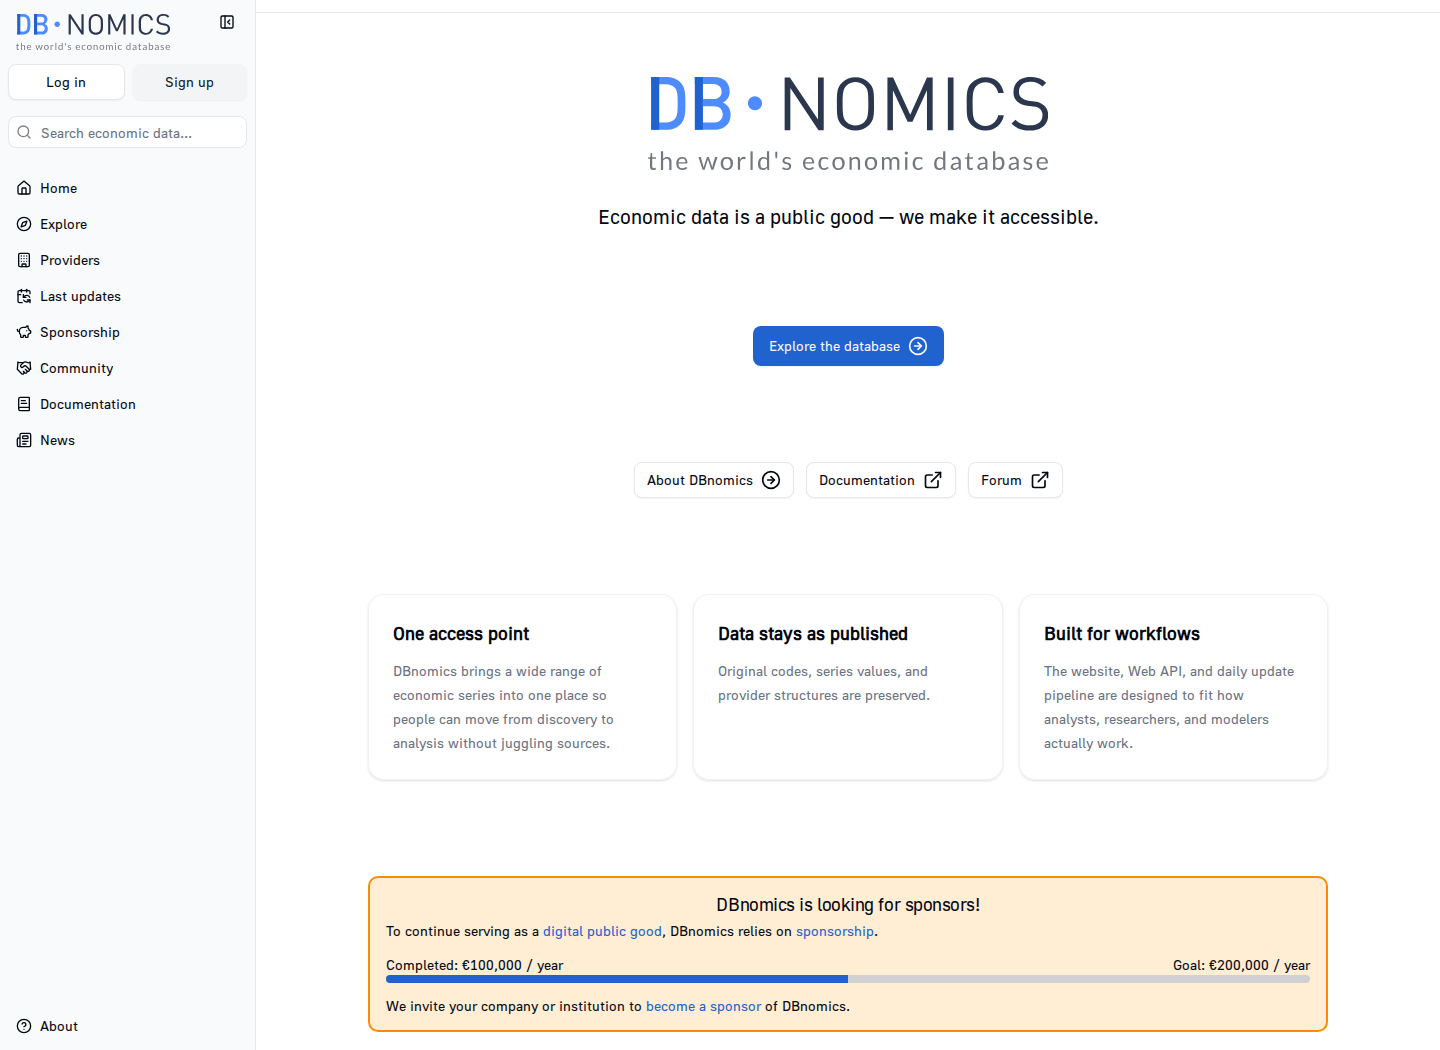
\includegraphics[width=.78\textwidth]{captures/dbnomics-home.png}\\
{\small DBnomics home page, captured on 11 November 2026.}
\end{center}

On the series page, the top breadcrumb identifies the provider and dataset.
The bracketed code before the title identifies the series within that dataset.
Read the full title, then use \emph{Chart}, \emph{Table}, \emph{Dimensions}
and \emph{Links} to inspect the observations, definitions and original source.
\emph{Download} exports data; \emph{Apply filters} opens a separate editor
and is not needed to retrieve the original observations in MATLAB.

\begin{center}
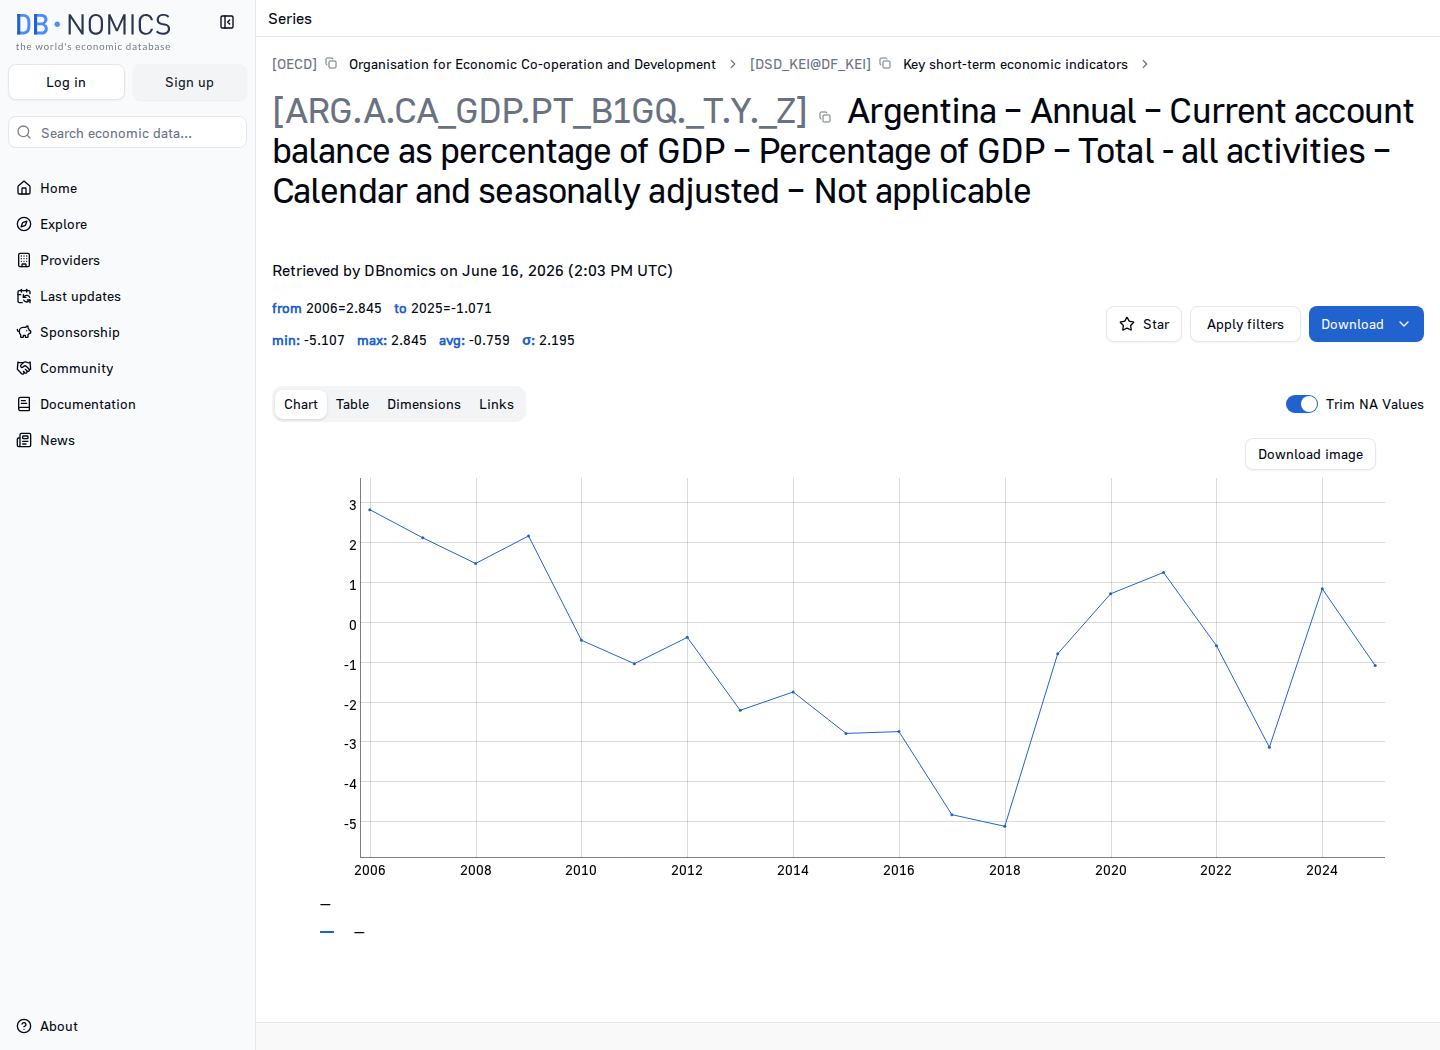
\includegraphics[width=.94\textwidth]{captures/dbnomics-series.png}\\
{\small OECD example, captured on 11 November 2026 (browser address bar not shown).}
\end{center}

\noindent\textbf{Page URL (shown explicitly, not part of the screenshot):}\\
\url{https://db.nomics.world/OECD/DSD_KEI@DF_KEI/ARG.A.CA_GDP.PT_B1GQ._T.Y._Z}

\noindent\textbf{Public series token to copy into MATLAB:}
\begin{minted}{matlab}
'OECD/DSD_KEI@DF_KEI/ARG.A.CA_GDP.PT_B1GQ._T.Y._Z'
\end{minted}
The token (also called a \emph{slug} or series identifier) is the complete
\texttt{provider/dataset/series} path after the website domain. Keep the
\texttt{@}, underscores, periods and capitalisation exactly as shown; omit
the domain and any query string. Here the provider is \texttt{OECD}, the
dataset is \texttt{DSD\_KEI@DF\_KEI}, and the final component is
\texttt{ARG.A.CA\_GDP.PT\_B1GQ.\_T.Y.\_Z}. Copying only that final component
is not enough for \texttt{call\_dbnomics}.

\textbf{This public token is not a secret API key or authentication token.}
The example is Argentina's annual current-account balance as a percentage of
GDP, not GDP growth. On 11 November 2026 the page and API both returned annual
observations from 2006 to 2025. Check these metadata again when reusing it.
For reproducibility, record the token, page URL, provider, access date,
frequency, units, transformations and missing-value treatment alongside code.

\clearpage
\section{Installation and first request}

The only MATLAB interface used in this note is \texttt{call\_dbnomics.m}.
Download the repository linked below. The function is in its \texttt{code/} folder; add that folder to the MATLAB path. In the standalone guide source folder, the same function is at the root. MATLAB must
have \texttt{webread}, \texttt{datetime}, \texttt{string} and Internet access. The examples are tested with MATLAB R2025a; no additional toolbox is required.\\
\url{https://github.com/Vermandel/dbnomics-teaching} No DBnomics account, API key or
credential is required.

\noindent\textbf{Direct download:} \href{https://raw.githubusercontent.com/Vermandel/dbnomics-teaching/1ff66c0c5d96b06556e5c0a202877cdc4a117d74/code/call_dbnomics.m}{\texttt{call\_dbnomics.m}} (required function).
Save it in a local \texttt{code/} folder and the examples linked below in a
sibling \texttt{examples/} folder. Keep the original filenames. These links
open raw files directly; if code is displayed, use the browser’s \emph{Save as}.
No account is needed.

\begin{minted}{matlab}
addpath('code') % from the downloaded repository root
[output_mat, output_table, dates_nb] = call_dbnomics( ...
    'Eurostat/prc_hicp_manr/M.RCH_A.TOT_X_NRG.AT');
\end{minted}

The function signature is
\begin{minted}{matlab}
[output_mat, output_table, dates_nb] = call_dbnomics(slug1, slug2, ...)
\end{minted}
If \texttt{RequestFailed} occurs, check the connection and retry the page in a browser: a temporary service failure does not establish that the token is wrong. If \texttt{InvalidSlug}, \texttt{MissingSeries} or \texttt{NoSeries} occurs, check the full three-part token.\par
All requested slugs must have the same frequency. The function downloads the
series, sorts their periods, aligns them on the union of dates and leaves a
missing observation as \texttt{NaN}.

\begin{itemize}
\item \texttt{output\_mat}: first column = MATLAB \texttt{datenum} dates;
remaining columns = observations.
\item \texttt{output\_table}: same observations in a MATLAB table; row names
are period labels and column names are the final dimension codes (for example
\texttt{AT} and \texttt{BE}). MATLAB makes repeated names unique.
\item \texttt{dates\_nb}: a readable numeric date vector: 2000, 2000.25,
2000.50 for quarterly data; $y+(m-1)/12$ for monthly data. Annual data use the year; daily data use MATLAB serial dates (not fractional years).
\end{itemize}

\section{One series}

\noindent\textbf{Download:} \href{https://raw.githubusercontent.com/Vermandel/dbnomics-teaching/1ff66c0c5d96b06556e5c0a202877cdc4a117d74/examples/example_single_series.m}{\texttt{example\_single\_series.m}}. Austrian inflation.

The first example downloads Austrian inflation. The second matrix column holds
the observations; its first column holds the dates.
\begin{minted}{matlab}
[mat, tab, dates] = call_dbnomics( ...
    'Eurostat/prc_hicp_manr/M.RCH_A.TOT_X_NRG.AT');
inflation_AT = mat(:,2);
\end{minted}
Inspect \texttt{tab(1:5,:)} and the last rows before transforming a series.
Do not confuse a rate of change, an index level and a seasonally adjusted level.

\section{Several countries}

\noindent\textbf{Download:} \href{https://raw.githubusercontent.com/Vermandel/dbnomics-teaching/1ff66c0c5d96b06556e5c0a202877cdc4a117d74/examples/example_multiple_countries.m}{\texttt{example\_multiple\_countries.m}}. Several countries in one request.

Within a dimension, \texttt{+} expands several codes. The following request,
from the historical examples, returns four columns: \texttt{AT}, \texttt{BE},
\texttt{DE} and \texttt{FR}.
\begin{minted}{matlab}
[mat, tab] = call_dbnomics( ...
    'Eurostat/prc_hicp_manr/M.RCH_A.TOT_X_NRG.AT+BE+DE+FR');
\end{minted}
If country coverage differs, the unmatched dates are represented by
\texttt{NaN}. A missing value is not zero: do not interpolate, forward-fill or
drop dates without a documented economic and statistical reason.

\section{Several series and alignment}

\noindent\textbf{Download:} \href{https://raw.githubusercontent.com/Vermandel/dbnomics-teaching/1ff66c0c5d96b06556e5c0a202877cdc4a117d74/examples/example_multiple_series.m}{\texttt{example\_multiple\_series.m}}. Aligned series and missing dates.

Pass several slugs as separate MATLAB arguments. This example requests two
monthly HICP measures for Austria and Germany:
\begin{minted}{matlab}
[mat, tab] = call_dbnomics( ...
    'Eurostat/prc_hicp_manr/M.RCH_A.TOT_X_NRG.AT+DE', ...
    'Eurostat/prc_hicp_manr/M.RCH_A.TOT_X_TBC.AT+DE');
complete = all(~isnan(mat(:,2:end)),2);
\end{minted}
The function does not silently aggregate or disaggregate. Download different
frequencies separately, then state and justify any conversion. Daily, monthly, quarterly and annual period conventions are supported; \texttt{UnsupportedFrequency} requires inspecting the actual period format. When names are
repeated, use \texttt{tab.Properties.VariableNames} to inspect the resulting
column names rather than assuming an order.

\clearpage
\section{Plotting}

Both scripts download exactly two monthly series: Austrian and Belgian HICP
annual inflation excluding energy. Their units and frequency are comparable.
The function aligns them on the sorted union of observation dates; matrix
columns 2 and 3 retain the order of the two arguments. Table values use that
same alignment. A missing value remains \texttt{NaN} and creates a gap in the
line: never replace it with zero merely to obtain a continuous plot.

\subsection*{A datetime time vector}
Download and run \href{https://raw.githubusercontent.com/Vermandel/dbnomics-teaching/1ff66c0c5d96b06556e5c0a202877cdc4a117d74/examples/example_plot_datetime.m}{\texttt{example\_plot\_datetime.m}} (two series, datetime axis). Convert the first matrix
column from MATLAB serial dates to \texttt{datetime}. Do not parse the table
row names with an assumed date format: their labels depend on frequency.
\inputminted[firstline=6]{matlab}{examples/example_plot_datetime.m}

\clearpage
\subsection*{A numeric time vector}
Download and run \href{https://raw.githubusercontent.com/Vermandel/dbnomics-teaching/1ff66c0c5d96b06556e5c0a202877cdc4a117d74/examples/example_plot_numeric.m}{\texttt{example\_plot\_numeric.m}} (two series, numeric axis). Here the third output is a
numeric vector $y+(m-1)/12$: January is $y$, February is $y+1/12$.
This is a readable monthly time scale, not a MATLAB \texttt{datenum}; do not
pass it to \texttt{datetick} or convert it with \texttt{ConvertFrom='datenum'}.
\inputminted[firstline=6]{matlab}{examples/example_plot_numeric.m}

Both examples use the returned dates, never a hand-made vector whose length
may differ from the downloaded sample. If a complete-case sample is needed,
apply the \emph{same} logical mask to time and to both value columns:
\begin{minted}{matlab}
keep = all(~isnan(mat(:,2:3)),2);
t_complete = t(keep);
y_complete = mat(keep,2:3);
\end{minted}
This removes incomplete rows; it is a substantive sample choice, not an
alignment repair. Inspect first and last dates, observation counts and units
before analysis, and cite the original provider as well as DBnomics.

\medskip\noindent{\small Legacy entry point: \href{https://raw.githubusercontent.com/Vermandel/dbnomics-teaching/1ff66c0c5d96b06556e5c0a202877cdc4a117d74/examples/example_plot_inflation.m}{\texttt{example\_plot\_inflation.m}}. This compatibility script runs \texttt{example\_plot\_datetime.m}; download both into the same \texttt{examples/} folder.}

\end{document}
